\documentclass[]{article}
\usepackage{lmodern}
\usepackage{amssymb,amsmath}
\usepackage{ifxetex,ifluatex}
\usepackage{fixltx2e} % provides \textsubscript
\ifnum 0\ifxetex 1\fi\ifluatex 1\fi=0 % if pdftex
  \usepackage[T1]{fontenc}
  \usepackage[utf8]{inputenc}
\else % if luatex or xelatex
  \ifxetex
    \usepackage{mathspec}
  \else
    \usepackage{fontspec}
  \fi
  \defaultfontfeatures{Ligatures=TeX,Scale=MatchLowercase}
\fi
% use upquote if available, for straight quotes in verbatim environments
\IfFileExists{upquote.sty}{\usepackage{upquote}}{}
% use microtype if available
\IfFileExists{microtype.sty}{%
\usepackage{microtype}
\UseMicrotypeSet[protrusion]{basicmath} % disable protrusion for tt fonts
}{}
\usepackage[margin=1in]{geometry}
\usepackage{hyperref}
\hypersetup{unicode=true,
            pdftitle={Homework 2},
            pdfauthor={Christophe Hunt},
            pdfborder={0 0 0},
            breaklinks=true}
\urlstyle{same}  % don't use monospace font for urls
\usepackage{color}
\usepackage{fancyvrb}
\newcommand{\VerbBar}{|}
\newcommand{\VERB}{\Verb[commandchars=\\\{\}]}
\DefineVerbatimEnvironment{Highlighting}{Verbatim}{commandchars=\\\{\}}
% Add ',fontsize=\small' for more characters per line
\usepackage{framed}
\definecolor{shadecolor}{RGB}{248,248,248}
\newenvironment{Shaded}{\begin{snugshade}}{\end{snugshade}}
\newcommand{\KeywordTok}[1]{\textcolor[rgb]{0.13,0.29,0.53}{\textbf{{#1}}}}
\newcommand{\DataTypeTok}[1]{\textcolor[rgb]{0.13,0.29,0.53}{{#1}}}
\newcommand{\DecValTok}[1]{\textcolor[rgb]{0.00,0.00,0.81}{{#1}}}
\newcommand{\BaseNTok}[1]{\textcolor[rgb]{0.00,0.00,0.81}{{#1}}}
\newcommand{\FloatTok}[1]{\textcolor[rgb]{0.00,0.00,0.81}{{#1}}}
\newcommand{\ConstantTok}[1]{\textcolor[rgb]{0.00,0.00,0.00}{{#1}}}
\newcommand{\CharTok}[1]{\textcolor[rgb]{0.31,0.60,0.02}{{#1}}}
\newcommand{\SpecialCharTok}[1]{\textcolor[rgb]{0.00,0.00,0.00}{{#1}}}
\newcommand{\StringTok}[1]{\textcolor[rgb]{0.31,0.60,0.02}{{#1}}}
\newcommand{\VerbatimStringTok}[1]{\textcolor[rgb]{0.31,0.60,0.02}{{#1}}}
\newcommand{\SpecialStringTok}[1]{\textcolor[rgb]{0.31,0.60,0.02}{{#1}}}
\newcommand{\ImportTok}[1]{{#1}}
\newcommand{\CommentTok}[1]{\textcolor[rgb]{0.56,0.35,0.01}{\textit{{#1}}}}
\newcommand{\DocumentationTok}[1]{\textcolor[rgb]{0.56,0.35,0.01}{\textbf{\textit{{#1}}}}}
\newcommand{\AnnotationTok}[1]{\textcolor[rgb]{0.56,0.35,0.01}{\textbf{\textit{{#1}}}}}
\newcommand{\CommentVarTok}[1]{\textcolor[rgb]{0.56,0.35,0.01}{\textbf{\textit{{#1}}}}}
\newcommand{\OtherTok}[1]{\textcolor[rgb]{0.56,0.35,0.01}{{#1}}}
\newcommand{\FunctionTok}[1]{\textcolor[rgb]{0.00,0.00,0.00}{{#1}}}
\newcommand{\VariableTok}[1]{\textcolor[rgb]{0.00,0.00,0.00}{{#1}}}
\newcommand{\ControlFlowTok}[1]{\textcolor[rgb]{0.13,0.29,0.53}{\textbf{{#1}}}}
\newcommand{\OperatorTok}[1]{\textcolor[rgb]{0.81,0.36,0.00}{\textbf{{#1}}}}
\newcommand{\BuiltInTok}[1]{{#1}}
\newcommand{\ExtensionTok}[1]{{#1}}
\newcommand{\PreprocessorTok}[1]{\textcolor[rgb]{0.56,0.35,0.01}{\textit{{#1}}}}
\newcommand{\AttributeTok}[1]{\textcolor[rgb]{0.77,0.63,0.00}{{#1}}}
\newcommand{\RegionMarkerTok}[1]{{#1}}
\newcommand{\InformationTok}[1]{\textcolor[rgb]{0.56,0.35,0.01}{\textbf{\textit{{#1}}}}}
\newcommand{\WarningTok}[1]{\textcolor[rgb]{0.56,0.35,0.01}{\textbf{\textit{{#1}}}}}
\newcommand{\AlertTok}[1]{\textcolor[rgb]{0.94,0.16,0.16}{{#1}}}
\newcommand{\ErrorTok}[1]{\textcolor[rgb]{0.64,0.00,0.00}{\textbf{{#1}}}}
\newcommand{\NormalTok}[1]{{#1}}
\usepackage{graphicx,grffile}
\makeatletter
\def\maxwidth{\ifdim\Gin@nat@width>\linewidth\linewidth\else\Gin@nat@width\fi}
\def\maxheight{\ifdim\Gin@nat@height>\textheight\textheight\else\Gin@nat@height\fi}
\makeatother
% Scale images if necessary, so that they will not overflow the page
% margins by default, and it is still possible to overwrite the defaults
% using explicit options in \includegraphics[width, height, ...]{}
\setkeys{Gin}{width=\maxwidth,height=\maxheight,keepaspectratio}
\IfFileExists{parskip.sty}{%
\usepackage{parskip}
}{% else
\setlength{\parindent}{0pt}
\setlength{\parskip}{6pt plus 2pt minus 1pt}
}
\setlength{\emergencystretch}{3em}  % prevent overfull lines
\providecommand{\tightlist}{%
  \setlength{\itemsep}{0pt}\setlength{\parskip}{0pt}}
\setcounter{secnumdepth}{5}
% Redefines (sub)paragraphs to behave more like sections
\ifx\paragraph\undefined\else
\let\oldparagraph\paragraph
\renewcommand{\paragraph}[1]{\oldparagraph{#1}\mbox{}}
\fi
\ifx\subparagraph\undefined\else
\let\oldsubparagraph\subparagraph
\renewcommand{\subparagraph}[1]{\oldsubparagraph{#1}\mbox{}}
\fi

%%% Use protect on footnotes to avoid problems with footnotes in titles
\let\rmarkdownfootnote\footnote%
\def\footnote{\protect\rmarkdownfootnote}

%%% Change title format to be more compact
\usepackage{titling}

% Create subtitle command for use in maketitle
\newcommand{\subtitle}[1]{
  \posttitle{
    \begin{center}\large#1\end{center}
    }
}

\setlength{\droptitle}{-2em}
  \title{Homework 2}
  \pretitle{\vspace{\droptitle}\centering\huge}
  \posttitle{\par}
  \author{Christophe Hunt}
  \preauthor{\centering\large\emph}
  \postauthor{\par}
  \predate{\centering\large\emph}
  \postdate{\par}
  \date{February 8, 2017}

\usepackage{relsize}
\usepackage{setspace}
\usepackage{amsmath,amsfonts,amsthm}
\usepackage[sfdefault]{roboto}
\usepackage[T1]{fontenc}
\usepackage{float}

\begin{document}
\maketitle

{
\setcounter{tocdepth}{2}
\tableofcontents
}
\section{Page 69: problem 12}\label{page-69-problem-12}

From this vague scenario, identify a problem you would like to study.
Which variables affect the behavior you have identified in the problem
identification? Which variables are the most important?

A company with a fleet of trucks faces increasing maintenance costs as
the age and mileage of the trucks increase.

A problem that would be interesting to study is the at what point should
the truck be retired and a new vehicle purchased. The costs associated
with a new purchase would need to outweigh the cost of maintaining the
aged truck. The variables of importance would be the maintenance cost as
its associated with the age and mileage of the truck, any additional
variables such as the severity of past repairs. I would assume that a
vehicle with engine failure may have future issues until the engine is
replaced, at which point the cost of maintenance may not be as severe.
Additionally, the cost of a new purchase would be the continuing
payments, depreciation, maintenance, fuel efficiency, and the
opportunity costs of reliability. The equilibrium of this system would
be meaningful to make a data driven decision to buy a new vehicle or to
keep running the aged truck.

\section{Page 79: problem 11}\label{page-79-problem-11}

Determine whether the data set supports the stated proportionality
model.

\[y \propto x^3\]

\begin{table}[!htbp]
\centering
\caption{}
\label{my-label}
\begin{tabular}{l|llllllllll}
y & 0 & 1 & 2 & 6 & 14 & 24 & 37 & 58 & 82 & 114 \\ \hline
x & 1 & 2 & 3 & 4 & 5 & 6 & 7 & 8 & 9 & 10
\end{tabular}
\end{table}

\begin{Shaded}
\begin{Highlighting}[]
\KeywordTok{library}\NormalTok{(ggplot2)}
\NormalTok{y <-}\StringTok{ }\KeywordTok{c}\NormalTok{(}\DecValTok{0}\NormalTok{, }\DecValTok{1}\NormalTok{, }\DecValTok{2}\NormalTok{, }\DecValTok{6}\NormalTok{, }\DecValTok{14}\NormalTok{, }\DecValTok{24}\NormalTok{, }\DecValTok{37}\NormalTok{, }\DecValTok{58}\NormalTok{, }\DecValTok{82}\NormalTok{, }\DecValTok{114}\NormalTok{)}
\NormalTok{x <-}\StringTok{ }\KeywordTok{c}\NormalTok{(}\DecValTok{1}\NormalTok{:}\DecValTok{10}\NormalTok{)}
\NormalTok{df <-}\StringTok{ }\KeywordTok{as.data.frame}\NormalTok{(}\KeywordTok{cbind}\NormalTok{(y,x))}
\NormalTok{df$y2 <-}\StringTok{ }\NormalTok{df$x^}\DecValTok{3}
\NormalTok{df$k <-}\StringTok{ }\NormalTok{df$y2/df$x}
\NormalTok{k <-}\StringTok{ }\KeywordTok{mean}\NormalTok{(df$k)}
\NormalTok{df$model <-}\StringTok{ }\NormalTok{k*df$x^}\DecValTok{3}



\KeywordTok{ggplot}\NormalTok{() +}\StringTok{ }
\StringTok{  }\KeywordTok{geom_line}\NormalTok{(}\DataTypeTok{data =} \NormalTok{df, }\KeywordTok{aes}\NormalTok{(x, y), }\DataTypeTok{color =} \StringTok{'red'}\NormalTok{) +}
\StringTok{  }\KeywordTok{geom_line}\NormalTok{(}\DataTypeTok{data =} \NormalTok{df, }\KeywordTok{aes}\NormalTok{(x,y2), }\DataTypeTok{color =} \StringTok{'blue'}\NormalTok{) +}
\StringTok{  }\KeywordTok{geom_line}\NormalTok{(}\DataTypeTok{data =} \NormalTok{df, }\KeywordTok{aes}\NormalTok{(x,model), }\DataTypeTok{color =} \StringTok{'green'}\NormalTok{) +}
\StringTok{  }\KeywordTok{theme_minimal}\NormalTok{() +}
\StringTok{  }\KeywordTok{ylim}\NormalTok{(}\DecValTok{10}\NormalTok{,}\DecValTok{10000}\NormalTok{)}
\end{Highlighting}
\end{Shaded}

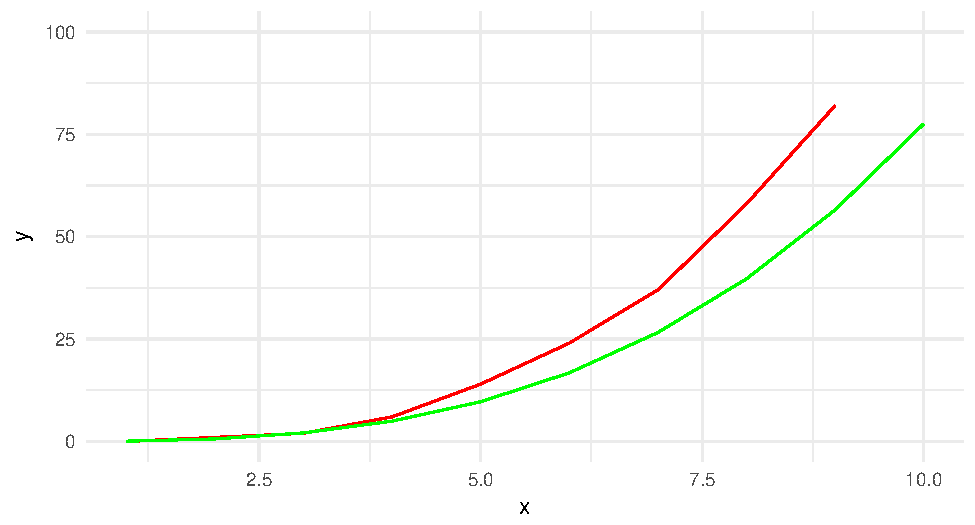
\includegraphics{CHunt_homework2_files/figure-latex/unnamed-chunk-1-1.pdf}

The data does not support the proportion model. Our used model for this
data is \(y = 38.5x^3\) where \(k = 38.5\). This is achieved by taking
\(y = x^3\) and substituting x for the values in our provided data set.
Then we obtain the ratio of \(y/x^3\) and further obtain the mean which
is \(38.5\). As illustrated above the model does not follow.

\section{Page 94: problem 4}\label{page-94-problem-4}

Lumber Cutters - Lumber cutters wish to use readily available
measurements to estimate the number of board feet for lumber in a tree.
Assume they measure the diameter of the tree in inches at waist height.
Develop a model that predicts board feet as a function of diameter in
inches.

Use the following data for your test.

\begin{table}[!htbp]
\centering
\caption{}
\label{my-label}
\begin{tabular}{l|llllllllll}
x & 17 & 19 & 20 & 23 & 25 & 28 & 32 & 38 & 39 & 41 \\ \hline
y & 19 & 25 & 32 & 57 & 71 & 113 & 123 & 252 & 259 & 294
\end{tabular}
\end{table}

The variable \(x\) is the diameter of a ponderous pine in inches, and y
is the number of board feet divided by 10.

\begin{enumerate}
\def\labelenumi{\alph{enumi}.}
\tightlist
\item
  Consider two separate assumptions, allowing each to lead to a model.
  Completely analyze each model.
\item
  Assume that all trees are right-circular cylinders and are
  approximately the same height.
\end{enumerate}

\begin{enumerate}
\def\labelenumi{\roman{enumi}.}
\setcounter{enumi}{1}
\tightlist
\item
  Assume that all trees are right-circular cylinders and that the height
  of the tree is proportional to the diameter.
\end{enumerate}

\begin{enumerate}
\def\labelenumi{\alph{enumi}.}
\setcounter{enumi}{1}
\tightlist
\item
  Which model appears to be better? Why? Justify your conclusions.
\end{enumerate}

\section{Page 99: problem 3}\label{page-99-problem-3}

Discuss several factors that were completely ignored in our analysis of
the gasoline mileage problem.

\section{Page 104: problem 2}\label{page-104-problem-2}

Tests exist to measure the percentage of body fat. Assume that such
tests are accurate and that a great many carefully collected data are
available. You may specify any other statistic, such as waist size and
height, that you would like collected. Explain how the data could be
arranged to check the assumptions underlying the sub models in this
section. For example, suppose the data for males between ages 17 and 21
with constant body fat and height are examined. Explain how the
assumption of constant density of the inner core could be checked.


\end{document}
